% Příčný řez dvoupólovým stejnosměrným strojem (schematicky).
% Kompilace: tectonic rez-stroje.tex  (XeTeX, písmo TeX Gyre Heros)
\documentclass[border=6pt]{standalone}
\usepackage{fontspec}
\setmainfont{texgyreheros}[Extension=.otf, UprightFont=*-regular, BoldFont=*-bold, ItalicFont=*-italic]
\usepackage{tikz}
\usetikzlibrary{arrows.meta,calc}

\definecolor{steel}{HTML}{E8E1D3}
\definecolor{ink}{HTML}{2B3033}
\definecolor{copper}{HTML}{C7763B}
\definecolor{lamel}{HTML}{E0B08A}
\definecolor{rotor}{HTML}{DCE5E3}
\definecolor{flux}{HTML}{E4572E}
\definecolor{spin}{HTML}{1F6B5C}
\definecolor{lead}{HTML}{5E676B}

\begin{document}
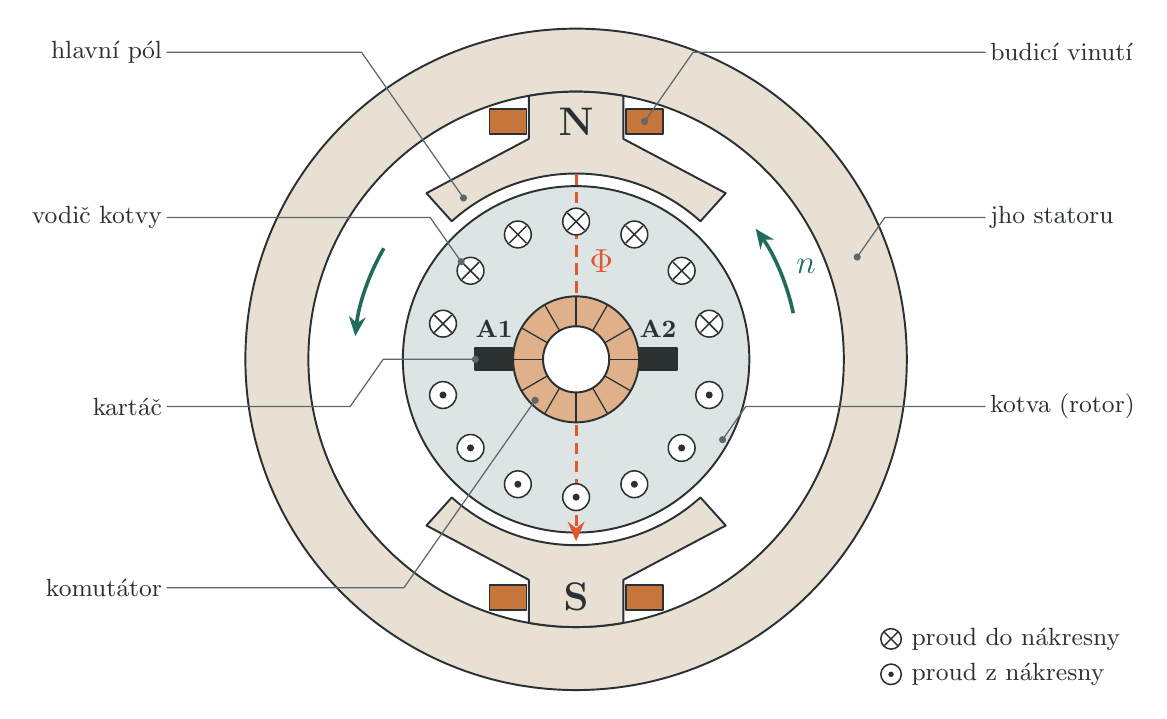
\begin{tikzpicture}[
  line join=round,
  body/.style={draw=ink, line width=0.7pt},
  % Odkazová čára: šikmý úsek k polici, vodorovná police, tečka na cíli
  leader/.style={draw=lead, line width=0.45pt},
  dot/.style={fill=lead, circle, inner sep=0pt, minimum size=2.6pt},
  lbl/.style={font=\small, text=ink, inner sep=1.5pt},
]
\def\Ro{4.2}  \def\Ri{3.4}   % jho statoru
\def\Ra{2.2}                  % kotva
\def\Rs{2.36}                 % líc pólového nástavce (vzduchová mezera)
\def\Rc{1.75}                 % poloměr drážek s vodiči

% --- Jho statoru
\fill[steel, even odd rule] (0,0) circle (\Ro) (0,0) circle (\Ri);
\draw[body] (0,0) circle (\Ro) (0,0) circle (\Ri);

% --- Hlavní póly (N nahoře, S dole): jádro dosedá na jho, dole pólový nástavec
%     Jedna uzavřená cesta: horní hrana kopíruje vnitřní obvod jha (r = 3,4).
\foreach \rot in {0,180} {
  \begin{scope}[rotate=\rot]
    \filldraw[body, fill=steel]
      (100.16:\Ri) arc[start angle=100.16, end angle=79.84, radius=\Ri]
      -- (0.6,2.8) -- (48:2.84) -- (48:\Rs)
      arc[start angle=48, end angle=132, radius=\Rs]
      -- (132:2.84) -- (-0.6,2.8) -- cycle;
    % budicí vinutí po stranách jádra, mimo jho i nástavec
    \filldraw[body, fill=copper] (0.63,2.86) rectangle (1.1,3.18);
    \filldraw[body, fill=copper] (-1.1,2.86) rectangle (-0.63,3.18);
  \end{scope}
}
\node[font=\bfseries\Large, text=ink] at (0,3.02) {N};
\node[font=\bfseries\Large, text=ink] at (0,-3.02) {S};

% --- Kotva
\filldraw[body, fill=rotor] (0,0) circle (\Ra);

% --- Magnetický tok Φ (pod komutátorem, aby ho nepřekrýval)
\draw[flux, line width=1.1pt, dash pattern=on 4pt off 2.5pt, -{Stealth[length=7pt,width=6pt]}]
  (0,\Rs) -- (0,-\Rs+0.05);
\node[text=flux, font=\large] at (0.32,1.25) {$\Phi$};

% --- Vodiče kotvy: nahoře proud do nákresny (⊗), dole z nákresny (⊙)
\foreach \a in {15,40,65,90,115,140,165} {
  \filldraw[body, fill=white, line width=0.55pt] (\a:\Rc) circle (0.17);
  \draw[ink, line width=0.55pt] ($(\a:\Rc)+(-0.11,-0.11)$) -- ($(\a:\Rc)+(0.11,0.11)$)
                                 ($(\a:\Rc)+(-0.11,0.11)$) -- ($(\a:\Rc)+(0.11,-0.11)$);
}
\foreach \a in {-15,-40,-65,-90,-115,-140,-165} {
  \filldraw[body, fill=white, line width=0.55pt] (\a:\Rc) circle (0.17);
  \fill[ink] (\a:\Rc) circle (0.045);
}

% --- Komutátor: 12 lamel, hřídel uprostřed
\filldraw[body, fill=lamel] (0,0) circle (0.8);
\foreach \a in {0,30,...,330} \draw[ink, line width=0.45pt] (\a:0.42) -- (\a:0.8);
\filldraw[body, fill=white] (0,0) circle (0.42);

% --- Kartáče v neutrální ose
\filldraw[body, fill=ink] (-1.28,-0.14) rectangle (-0.8,0.14);
\filldraw[body, fill=ink] (0.8,-0.14) rectangle (1.28,0.14);
\node[font=\bfseries\small, text=ink] at (-1.04,0.38) {A1};
\node[font=\bfseries\small, text=ink] at (1.04,0.38) {A2};

% --- Smysl otáčení n (proti směru hodinových ručiček)
%     Šipky leží ve vzduchové mezeře v úsecích, kudy nevede žádná odkazová čára.
\draw[spin, line width=1.3pt, -{Stealth[length=7pt,width=6pt]}]
  (12:2.82) arc[start angle=12, end angle=36, radius=2.82];
\draw[spin, line width=1.3pt, -{Stealth[length=7pt,width=6pt]}]
  (150:2.82) arc[start angle=150, end angle=174, radius=2.82];
\node[text=spin, font=\large] at (22:3.15) {$n$};

% --- Odkazové čáry
%     Popisky leží vlevo i vpravo na společných řádcích (y = 3,9 / 1,8 / -0,6 / -2,9).
%     Každá čára má šikmý úsek pod stejným úhlem 55° a vodorovnou polici ke sloupci
%     textu. Na každé straně jdou cíle shora dolů ve stejném pořadí jako řádky,
%     takže se čáry nekříží.
\def\Col{5.2}   % sloupec textu (|x|)
\def\Ang{55}    % sklon šikmého úseku
\newcommand{\leaderline}[5]{% #1 strana (-1/1), #2 x cíle, #3 y cíle, #4 y řádku, #5 text
  \pgfmathsetmacro{\ex}{#2 + #1*abs(#4-#3)/tan(\Ang)}
  \draw[leader] (#2,#3) -- (\ex,#4) -- (#1*\Col,#4);
  \node[dot] at (#2,#3) {};
  \ifnum#1<0 \node[lbl, anchor=east] at (#1*\Col,#4) {#5};
  \else      \node[lbl, anchor=west] at (#1*\Col,#4) {#5}; \fi
}
% Varianta s vodorovným výběhem: cíl leží mezi vodiči kotvy, šikmý úsek začne až za kotvou.
\newcommand{\leaderjog}[6]{% #1 strana, #2 x, #3 y, #4 y řádku, #5 text, #6 x konce výběhu
  \pgfmathsetmacro{\ex}{#6 + #1*abs(#4-#3)/tan(\Ang)}
  \draw[leader] (#2,#3) -- (#6,#3) -- (\ex,#4) -- (#1*\Col,#4);
  \node[dot] at (#2,#3) {};
  \node[lbl, anchor=east] at (#1*\Col,#4) {#5};
}
% vlevo
\leaderline{-1}{-1.43}{2.05}{3.9}{hlavní pól}
\leaderline{-1}{-1.46}{1.24}{1.8}{vodič kotvy}
\leaderjog{-1}{-1.28}{0.00}{-0.6}{kartáč}{-2.45}
\leaderline{-1}{-0.52}{-0.52}{-2.9}{komutátor}
% vpravo
\leaderline{1}{0.87}{3.02}{3.9}{budicí vinutí}
\leaderline{1}{3.57}{1.30}{1.8}{jho statoru}
\leaderline{1}{1.86}{-1.02}{-0.6}{kotva (rotor)}

% --- Legenda směru proudu (bez odkazových čar)
\begin{scope}[shift={(4.0,-3.55)}]
  \filldraw[body, fill=white, line width=0.55pt] (0,0) circle (0.13);
  \draw[ink, line width=0.5pt] (-0.085,-0.085) -- (0.085,0.085) (-0.085,0.085) -- (0.085,-0.085);
  \node[lbl, anchor=west] at (0.2,0) {proud do nákresny};
  \filldraw[body, fill=white, line width=0.55pt] (0,-0.45) circle (0.13);
  \fill[ink] (0,-0.45) circle (0.035);
  \node[lbl, anchor=west] at (0.2,-0.45) {proud z nákresny};
\end{scope}
\end{tikzpicture}
\end{document}
